% Options for packages loaded elsewhere
\PassOptionsToPackage{unicode}{hyperref}
\PassOptionsToPackage{hyphens}{url}
%
\documentclass[
]{article}
\usepackage{lmodern}
\usepackage{amssymb,amsmath}
\usepackage{ifxetex,ifluatex}
\ifnum 0\ifxetex 1\fi\ifluatex 1\fi=0 % if pdftex
  \usepackage[T1]{fontenc}
  \usepackage[utf8]{inputenc}
  \usepackage{textcomp} % provide euro and other symbols
\else % if luatex or xetex
  \usepackage{unicode-math}
  \defaultfontfeatures{Scale=MatchLowercase}
  \defaultfontfeatures[\rmfamily]{Ligatures=TeX,Scale=1}
\fi
% Use upquote if available, for straight quotes in verbatim environments
\IfFileExists{upquote.sty}{\usepackage{upquote}}{}
\IfFileExists{microtype.sty}{% use microtype if available
  \usepackage[]{microtype}
  \UseMicrotypeSet[protrusion]{basicmath} % disable protrusion for tt fonts
}{}
\makeatletter
\@ifundefined{KOMAClassName}{% if non-KOMA class
  \IfFileExists{parskip.sty}{%
    \usepackage{parskip}
  }{% else
    \setlength{\parindent}{0pt}
    \setlength{\parskip}{6pt plus 2pt minus 1pt}}
}{% if KOMA class
  \KOMAoptions{parskip=half}}
\makeatother
\usepackage{xcolor}
\IfFileExists{xurl.sty}{\usepackage{xurl}}{} % add URL line breaks if available
\IfFileExists{bookmark.sty}{\usepackage{bookmark}}{\usepackage{hyperref}}
\hypersetup{
  hidelinks,
  pdfcreator={LaTeX via pandoc}}
\urlstyle{same} % disable monospaced font for URLs
\usepackage[margin=1in]{geometry}
\usepackage{graphicx,grffile}
\makeatletter
\def\maxwidth{\ifdim\Gin@nat@width>\linewidth\linewidth\else\Gin@nat@width\fi}
\def\maxheight{\ifdim\Gin@nat@height>\textheight\textheight\else\Gin@nat@height\fi}
\makeatother
% Scale images if necessary, so that they will not overflow the page
% margins by default, and it is still possible to overwrite the defaults
% using explicit options in \includegraphics[width, height, ...]{}
\setkeys{Gin}{width=\maxwidth,height=\maxheight,keepaspectratio}
% Set default figure placement to htbp
\makeatletter
\def\fps@figure{htbp}
\makeatother
\setlength{\emergencystretch}{3em} % prevent overfull lines
\providecommand{\tightlist}{%
  \setlength{\itemsep}{0pt}\setlength{\parskip}{0pt}}
\setcounter{secnumdepth}{-\maxdimen} % remove section numbering

\author{}
\date{\vspace{-2.5em}}

\begin{document}

\hypertarget{introduction}{%
\section{Introduction}\label{introduction}}

\hypertarget{problem-description}{%
\subsection{Problem Description}\label{problem-description}}

wetlands are the most threatened and least protected ecosystems globally
and in South Africa {[}@skownoNationalBiodiversityAssessment2019{]}.
Wetlands are areas where the land is covered with water such as marshes,
sedges, river deltas, edges of lakes or oceans, etc. Wetlands benefit
society in many ways. These include flood control, storm buffering and
water quality improvement {[}@clarksonWetlandEcosystemServices2013{]}.
Wetlands are invaluable to society and their surrounding communities.

The threat to wetlands has only recently been realised locally. Wetland
conservation programs for South Africa have been created as late as 2002
despite the severe wetland degradation experienced over the years. As a
result of the relative late response, 35-60\% of South Africa's wetlands
have been severely damaged or destroyed due to bad agricultural
practices {[}@departmentofenvironmentalaffairsWorkingWetlands2019{]}. As
a result, there have been recent programs for wetland rehabilitation.
Most notably, the Working for Wetlands, initiated in 2002. Working for
Wetlands was initiated by the Water Research Commission, in partnership
with the Department of Environmental Affairs, and aims to rehabilitate
and protect wetlands in South Africa.

Destruction or degradation of an ecosystem leads to a decrease in
species populations and/or a decrease in biodiversity. According to the
WWF's 2018 living planet report, it's stated that there's been a 60\%
decrease in global population biodiversity of mammals, fish, birds,
reptiles and amphibians {[}@grootenLivingPlanetReport2018{]}. These
views are supported by the Living Planet Index (LPI). As a result, there
has been a notable increase in effort to preserve and recover global
biodiversity. The most notable being The Aichi Biodiversity targets. The
Aichi Convention on Biological Diversity presented a strategic plan in
2011 to improve global biodiversity. This plan is made up of 5 goals and
20 targets. The strategic plan needed appropriate metrics to measure its
success, and as a result the Living Planet Index (LPI) was created. The
LPI measures the progress of Aichi strategic goal C. Aichi strategic
goal C states: ``To improve the status of biodiversity by safeguarding
ecosystems, species and genetic diversity''
{[}@conventiononbiologicaldiversityAichiBiodiversityTargets2020{]}.

Biodiversity is invaluable to our ecosystems and society at large. With
loss of biodiversity comes reduced ecosystem resilience
{[}@ritchieBiodiversity2021{]}. It's thus imperative to keep track of an
ecosystem's biodiversity and species population dynamics to understand
the state of an ecosystem. One of the best tools to track biodiversity
and species population dynamics are birds
{[}@amatWaterbirdsBioindicatorsEnvironmental2010;
@mekonenBirdsBiodiversityEnvironmental2017{]}. Consequently, a citizen
scientist initiative, called the Coordinated Waterbird Counts (CWAC),
was initiated in 1992 by the Animal Demographic Unit (ADU), to keep
track of bird counts in wetlands around South Africa. The CWAC dataset
has bird counts of over 200 different bird species from approximately
400 different wetland locations in South Africa. Some of these counts go
back as far as the 1970s.

Wetlands and waterbirds are the subject of many conservation projects
locally and worldwide. Organisations involved include Agreement on the
Conservation of African-Eurasian Migratory Waterbirds (AEWA), Convention
on Wetlands of International Importance Especially as Waterfowl Habitat
(RAMSAR) and the Working for Wetlands initiative. Regarding the
waterbirds in South Africa, there is currently a robust citizen-science
based bird count data in the form of the CWAC dataset. Unfortunately,
this is a raw dataset and not very accessible to the broader community.
The aim of this project is to use the raw CWAC dataset and produce
concise and effective data products, using various statistical
techniques, that can be used by experts and non-experts to understand
the state of the wetland and waterbird species of South Africa.

\hypertarget{background-to-research}{%
\subsection{Background to Research}\label{background-to-research}}

My project forms part of a larger project, The South Africa BiodIveRsity
Data pIpelinE for wetlands and waterbirds (BIRDIE)
\url{https://www.sanbi.org/biodiversity/building-knowledge/biodiversity-monitoring-assessment/freshwater-programme-birdie-project}.
BIRDIE is a project that aims to collate all types of wetland data,
perform statistical analysis, and make the output available to the
public. The data pipeline is to utilise raw wetland data, collate it and
produce data that is directly useful for decision making purposes on a
local and global scale.

The output will be relevant at national, regional and local levels. At
the national level, The data output provides insights of the state of
South African wetlands and waterbirds that can be used by international
conservation projects like AEWA and Ramsar. At the regional level, the
data output supports provincial conservation agencies who need to make a
range of decisions about the conservation of sites and species. For
example, Some species are hunted and quotas need to be set. At the local
level, The data output aids wetland site managers decision making
regarding the preservation of the wetland and its bird species.
Furthermore, the output is also beneficial to keen bird watching
enthusiasts in helping identify which bird species are present at which
wetlands.

The BIRDIE project is being conducted by the South African National
Biodiversity Institute (SANBI), in association with FitzPatrick
Institute for African Ornithology (FIAO, UCT), the Centre for Statistics
in Ecology, Environment and Conservation (SEEC at the University of Cape
Town), Seascape Belgium and the Royal Belgium Institute of Natural
Sciences (RBINS). The end goal is to provide automated statistical
computing processes on raw data and produce effective visualisations and
other data specific output hosted on a web app.

One of the key datasets in the BIRDIE project is the CWAC dataset. The
CWAC dataset is well managed and maintains standard protocols for the
counters to ensure reliable counts. The census data captured are also
presented to international biodiversity contributors such as AEWA and
the RAMSAR convention.

CWAC counts usually take place twice a year. Once in summer,
traditionally during January and February, and once in winter,
traditionally during July. The counting protocol is standardised to
increase reliability of the counts and the ability to compare counts
across different wetland sites. Counters are encouraged to adhere to
these methods as closely as possible. Variables such as number of
counters, routes followed, time of day, tide, viewing technique, viewing
aids, personnel and counting technique are all kept constant for each
wetland. Due to varying terrains and environments, each wetland may
require slightly different counting techniques, but these techniques
remain constant once established {[}@aduCWACCoordinatedWaterbird2020{]}.
Further information on the CWAC counting procedure can be found on the
CWAC website (\url{http://www.adu.org.za/docs/cwac-info4.pdf}).

The CWAC dataset provides an important insight into the state of
wetlands across South Africa. Unfortunately, the data is raw and
difficult to analyse by non-experts. Analysing the count data and
identifying pattens in species abundance, biodiversity and population
dynamics over the years is an important step in identifying wetland
state and to measure if wetland rehabilitation programs have been
working.

\hypertarget{state-space-time-series-model-ssm}{%
\subsection{State space time series model
(SSM)}\label{state-space-time-series-model-ssm}}

State space models (SSMs) have become a popular tool used by ecologists
to analyse ecological time-series. There is enough evidence to argue
that SSMs should be the default tool in analysing time series for
ecologists {[}@auger-metheGuideStatespaceModeling2021{]}. SSMs have been
used in various ecological studies such as fisheries stock assessment
{[}@aeberhardRobustEstimationDiscretetime2020{]}, movement ecology
{[}@pattersonStateSpaceModels2008{]} and, most commonly, modelling
population dynamics {[}@newmanStateSpaceModels2014{]}. These are only a
few examples of where SSMs are used. Their application in ecology is
vast.

SSMs are able to model temporal autocorrelation in a way that separates
observation error from process error
{[}@auger-metheGuideStatespaceModeling2021{]}. Herein lies the value of
SSMs. SSMs are hierarchical models that essentially model two different
time series. One being the state process (latent process or hidden
process) which is the unobserved time series that represents the true
underlying population dynamics. The other being the observation process
that represents the observed counts of that state process. Count data is
often prone to observation error, especially when counting large groups
of birds. Therefore, separating the observation process from the state
process provides a more accurate estimation of the true population. The
beauty in this methodology is that variation attributed to population
size, population growth rate, environmental stochasticity and any other
forms of stochasticity can be estimated from the model
{[}@keryBayesianPopulationAnalysis2011{]}. This allows the ecologist to
program the state space time series model such that it accounts for
known biological factors that affect the population dynamics. This
includes birth rates, death rates, fecundity, immigration, emigration,
etc. Figure 1 shows a simple visual illustration of this separation
between state and observation processes.

\begin{figure}[H]
  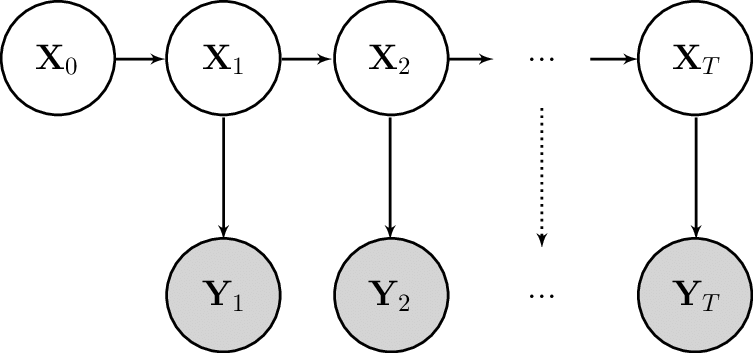
\includegraphics{D:/Thesis/birdie/Report/img/The-state-space-model.png}
  \caption{A visual representation of a state space model where $X_t$ is the true population state and $Y_t$ is the observations}
\end{figure}

When applying SSMs to count data there are two important conditions that
must be met for the SSM to produce unbiased estimates of population
size. Firstly, false negative (false detections) and false positive
(double counting) observations should cancel out on average. Secondly,
there should be no temporal patterns in detection probability or false
positive rates over time {[}@keryBayesianPopulationAnalysis2011{]}.

\hypertarget{bioindicators}{%
\subsection{Bioindicators}\label{bioindicators}}

Fitting SSMs to population data helps us understand how the population
of individual species have fluctuated over the years. But these models
don't tell the viewer much about the biodiversity of the ecosystem. This
is where bioindicators and indices come in. In this report,
bioindicators refer to biological aspects of an ecosystem that reflect
changes in the ecosystem. For example, birds are good organisms to use
as bioindicators as they reflect various environmental changes directly
{[}@mekonenBirdsBiodiversityEnvironmental2017{]}. Indices, in this
report, refer to summarised information. The LPI is an example of such
an index as it aggregates multiple species trends into a single index
value.

Environmental assessments play an important role in environmental
decision-making. This has lead to a stark increase in assessment reports
that are based on bioindicators
{[}@niemeijerFramingEnvironmentalIndicators2008{]}. According to
@niemeijerFramingEnvironmentalIndicators2008, the bioindicators used in
these reports often follow a common causal chain. This means that the
bioindicator in use directly reflect specific changes in an ecosystem.
For example, a decrease in wetland water level would be reflected in the
declining population of waterbird species of that wetland
{[}@burgessHabitatManagementMidContinent1969{]}.
@niemeijerFramingEnvironmentalIndicators2008 argue that the
bioindicators used are too specific. One should instead use
bioindicators that reflect multiple changes in an ecosystem. Bird
species are ideal bioindicators to use as they reflect many aspects of
an ecosystem {[}@mekonenBirdsBiodiversityEnvironmental2017{]}

According to @gregoryUsingBirdsIndicators2003, effective bioindicators
are quantitative, easy to collect, simple to interpret, reflect causes
of change in an ecosystem and indicate general patterns of taxa in the
ecosystem. Bird count data fits this well. As bird counts are relatively
easy to collect (and readily available), quantitative, simple to
interpret and they reflect multiple different changes in an ecosystem.

Birds have been used to indicate the eutrophication levels in wetlands
in the Mar Menor lagoon of south-eastern Spain
{[}@amatWaterbirdsBioindicatorsEnvironmental2010{]}. It was discovered
that the Great Crested Grebe abundance increased as the eutrophication
levels in the lagoon increased. The increase in eutrophication was a
result of nutrient run-off from nearby agricultural practices. Another
example from Southern Spain shows the use of Red-Knobbed Coots to
indicate the siltation rate in the water and soil in wetlands
{[}@amatWaterbirdsBioindicatorsEnvironmental2010{]}. The Red-Knobbed
Coot experienced a stark decline in abundance in the 20th century in
Southern Spain. This decrease in abundance is attributed to the
increased siltation rates in the water and soil in the wetlands in
Southern Spain. Caused by invasive agricultural practices. The increased
rates of siltation negatively affected the quality of food for the Coots
in their wetlands, and thus lead to their demise. Thus, the Red-Knobbed
Coots population over time could be indicative of siltation rates in the
wetlands in which they are based. These are only two examples of how
effective waterbirds are as bioindicators. Other examples show how
waterbirds can be indicators for changes in water level in a wetland
{[}@burgessHabitatManagementMidContinent1969{]} and species abundance at
lower trophic levels {[}@mekonenBirdsBiodiversityEnvironmental2017{]}.

An important aspect of ecosystem health is biodiversity. Rich
biodiversity is indicative of a healthy ecosystem. Each species has
their part to play in the ecosystem with varying degrees of importance.
Tracking biodiversity in an ecosystem can also indicate the presence of
invasive species {[}@hooperEffectsBiodiversityEcosystem2005{]}.
Biodiversity indicators are therefore essential in tracking the overall
health of a wetland ecosystem.

Two of the more common biodiversity indicators are the Shannon's entropy
and the Simpson's index. The exponentiated Shannon's entropy reflects
the effective number of species types in an ecosystem based on the
species counts {[}@jostEntropyDiversity2006{]}. The Simpson's index
presents a measure of evenness in a community with 1 being perfect
evenness and 0 being very poor evenness. Evenness refers to how the
waterbird counts are distributed across the waterbird species. If a
community has equal counts for each species the Simpson's index would be
1 and the community of waterbird species would be perfectly even. If
there are one or two species that have significantly higher counts than
the rest, then the Simpson's index would be closer to 0 indicating that
the community is uneven, and some species are dominant in the ecosystem.

There are currently various indicators used, worldwide, that aggregate
and measure species trends. These are used to provide an overview of the
species health in an ecosystem. The main index in use, globally, is the
Living Planet Index (LPI) {[}@collenMonitoringChangeVertebrate2009{]}.
There are other similar indices such as the Australian Threatened
Species Index (TSX) {[}@bayraktarovThreatenedSpeciesIndex2020{]} and the
Wild Bird Index (WBI) {[}@gregoryWildBirdIndicators2010{]}. Both the TSX
and the WBI are based on the calculations used by the LPI.

Choosing the best index to use proved to be a difficult task as decision
science has rarely been applied to these global indices to evaluate
their effectiveness and their design
{[}@watermeyerUsingDecisionScience2021{]}. However, a study by
@watermeyerUsingDecisionScience2021 was conducted that applied decision
science techniques to 9 different, commonly used, global environmental
indicies, one being the LPI. Based on the study, the LPI performed well
in 4 of the 5 criteria used. The criteria being: How well the index
meets its objectives, design, behaviour, methods to test uncertainty,
and feasibility. The LPI performed well in all aspects except for
feasability.

The LPI was initiated in 1997 by the WWF and the World Conservation
Monitoring Centre. It is the most used index that monitors average
vertebrate trends around the world. These trend estimates are based on
data from as far back as 1970. It uses time-series data from around the
world and aims to measure the state of the world's population trends of
vertebrate species. The Index covers the terrestrial, freshwater and
marine habitats. The time series data is further broken up into its
specific biomes and geographic realms or oceans.

\hypertarget{aim-and-objectives}{%
\subsection{Aim and Objectives}\label{aim-and-objectives}}

The CWAC dataset is currently a raw and hard to access dataset. The aim
of this study is to extract relevant information from the data in the
form of time series analysis and bioindicators to track bird species
population dynamics and biodiversity. State space time series models
(SSM) are used to model the population dynamics. SSMs have become
popular amongst ecologists when dealing with population dynamics and is
fast becoming the norm {[}@auger-metheGuideStatespaceModeling2021{]}.
SSMs work well with count data as they separate the observation error
from the process error {[}@keryBayesianPopulationAnalysis2011{]}. This
gives the ecologist a better understanding of the true population
dynamics. SSMs are also good for forecasting future values or missing
values which is suitable for the CWAC dataset as it contains missing
counts for some years. The SSM is key to the following aims as the
posterior sample is used for further calculations to develop
bioindicators.

When formulating bioindicators from data, it's important to first
understand what needs to be monitored
{[}@yoccozMonitoringBiologicalDiversity2001{]}. Given the context of
wetland and waterbird conservation, multiple types of indicators were
necessary to produce a wholistic view of the state of the wetland and
waterbirds present. The bioindicators developed using the CWAC dataset
were the exponentiated Shannon's entropy, the Simpson's index and a
modified Living Planet Index (LPI).

Wetland and waterbird conservationists will be able to utilise these
indices and time series models to understand the state of the wetland in
terms of its bird species. Furthermore, it can be used as a tool by
AEWA, Ramsar and the common bird enthusiast, to monitor the waterbird
species in South Africa. The Barberspan wetland is used as pilot study,
but if successful, this analysis can be used on all wetland sites
represented in the CWAC dataset.

The following are the objectives that, if followed, will lead to
successful completion of the aim:

\begin{enumerate}
\def\labelenumi{\arabic{enumi}.}
\tightlist
\item
  Research and develop relevant state space time series model for bird
  population dynamics in Barberspan. These models can be used for
  understanding the change of bird counts over time and forecasting
  future values.
\item
  Identify species attributes that may affect the population dynamics.
\item
  Formulate relevant biodiversity indicators using the output of the
  state space model.
\item
  Formulate both the state space models and biodiversity indicators such
  that they display a good overview of wetland state that can be used by
  both non-experts and experts.
\end{enumerate}

\end{document}
